\begin{figure}
    \centering
\begin{knitrout}
\definecolor{shadecolor}{rgb}{0.969, 0.969, 0.969}\color{fgcolor}\begin{kframe}


{\ttfamily\noindent\bfseries\color{errorcolor}{\#\# Error: Faceting variables must have at least one value}}\end{kframe}
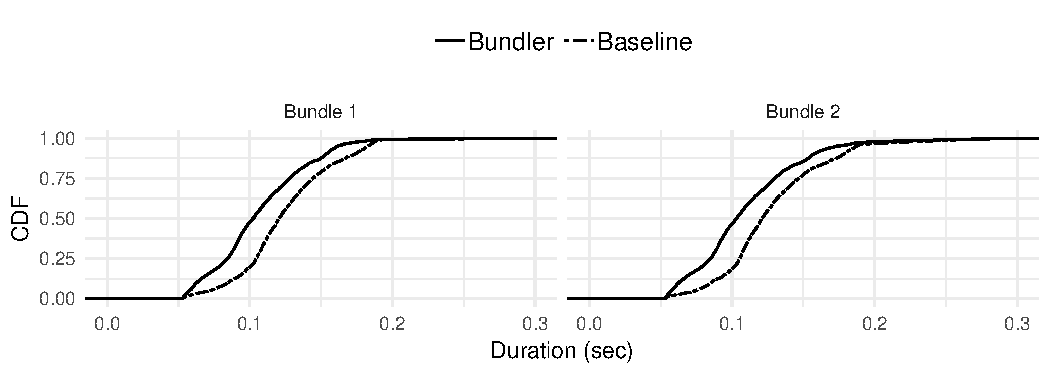
\includegraphics[width=\maxwidth]{figure/robust:twobundler-1} 

\end{knitrout}
    \caption{Competing traffic bundles. In both cases, the aggregate offered load is 84Mbps, as in Figure~\ref{fig:eval:best}. For "1:1", we evenly split the offered load between the two Bundles; for "2:1", one bundle has twice the offered load of the other. In both cases, each bundle observes improved median FCT compared to its performance in the baseline scenario.}
    \label{fig:robust:twobundler}
\end{figure}
